\documentclass[a4paper,floatfix,twocolumn,preprintnumbers,superscriptaddress]{article}%twoside
\usepackage{packages/xjenzaP}
\usepackage{datetime,tabularx,multirow,subfigure,dblfloatfix}
\usepackage{graphicx,float}
\usepackage{fancyhdr,calc}
\usepackage[hidelinks]{hyperref}
\usepackage{lipsum,cuted,setspace,enumerate}
\usepackage[ansinew,utf8]{inputenc}
\usepackage[compact]{titlesec}
\usepackage{changepage}
\usepackage{xcolor,colortbl,color}
\usepackage{soul,hyphenat}
\usepackage{algpseudocode}
\usepackage{algorithm}
\usepackage{textgreek, upgreek, tipa}% these should be before amssymb, amsthm and amsmath
\usepackage{amssymb,amsthm}
\usepackage{relsize}
\usepackage{epstopdf}
\usepackage{siunitx}
\usepackage{mhchem}
\usepackage{booktabs}
\usepackage{balance}
\usepackage{enumitem}
\usepackage{placeins}
\setlist{noitemsep}
\usepackage{latexsym}
\usepackage{pdfpages}
\usepackage{multicol}
%\usepackage{flushend}%balancing cols

%--Settings for the modified apa citation style--:::::::::::::::::::::::::::::::::
%
%  This method uses the Biblatex package with the biber backend.
%  After installing the Biblatex package install the 
%  biblatex-apa citation style. Afterwords, replace the `apa.bbx'
%  and `apa.cbx' files in the biblatex-apa directory, ex:
%  /usr/local/share/texmf/tex/latex/biblatex-apa
%  with the files present in the packages folder.

\usepackage[british]{babel}
\usepackage[isbn=false,url=false,doi=false,eprint=false,sorting=nyt, backend=biber, style=xjenza]{biblatex}
%\usepackage[sorting=nyt, backend=biber, style=apa]{biblatex}
\AtEveryBibitem{% suppressing the month
  \clearfield{month}
  \clearfield{day}
}
\DeclareLanguageMapping{british}{british-apa}
%---

%--Item spacing: add \begin{enumerate}[noitemsep,topsep=0pt,
%--parsep=0pt,partopsep=0pt] to use--:::::::::::::::::::::::::::::::::::::::::::::

\usepackage{enumitem}
\setitemize{noitemsep,topsep=0pt,parsep=0pt,partopsep=0pt}
%---

%--New commands--:::::::::::::::::::::::::::::::::::::::::::::::::::::::::::::::::
\newcommand{\udt}[3]{#1^{#2}_{\phantom{#2}#3}}
\newcommand{\dut}[3]{#1_{#2}^{\phantom{#2}#3}}
\newcommand{\dudt}[4]{#1_{#2\phantom{#3}#4}^{\phantom{#2}#3}}
%---

%--section white space--::::::::::::::::::::::::::::::::::::::::::::::::::::::::::
\titlespacing{\section}{0pt}{*1}{*1}
\titlespacing{\subsection}{0pt}{*1}{*1}
\titlespacing{\subsubsection}{0pt}{*1}{*1}
%---

%--paragraph spacing--::::::::::::::::::::::::::::::::::::::::::::::::::::::::::::
\parindent 10 pt
\parskip 0 pt
%---

%::::::::::::::::::::::::--End of xjenza-preamble.tex--::::::::::::::::::::::::::%

\title{Sample paper on how to use the \LaTeX{} Xjenza template}
\doi{DOI}
\articleType{Sample Article}%Research Article, Review Article, Research Note, News Article...
\author{W. Hicklin$^1$, J. Levi Said$^2$}
\authorAnnotation{$^1$University of Malta, Department of Physics\\
$^2$University of Malta, Department of Physics}
\correspondanceName{W. Hicklin}
\correspondanceMail{xjenza.copy.editor@gmail.com}

\addbibresource{bibliography.bib}

% Space for additional packages




\setcounter{page}{1}

\begin{document}
\abstrac{This is a sample paper to help you get use to the Xjenza template. Throughout this document one should find conventions on how to write chemical formula, tables, units, figures and equations using LaTeX. Furthermore, examples will be given on how to do citations and text citations.}

\maketitle

\section{Introduction}

The following is some Latin text to give you an idea of the type setting of the template.

\lipsum[1-3]

\section{Chemical formula}

Writing chemical formulas is made easy with the mhchem package. Here are a couple of examples:

\ce{2H2O -> 4H2 + O2}

\ce{->}

\ce{<-}

\ce{<=>}

\ce{<->}

\ce{->[{Process}]}

\ce{CH3\sbond C\tbond C\dbond CH2}

\begin{equation}
\ce{AgCl <=> Ag+ + Cl-}
\end{equation}

%\begin{strip}
\begin{equation}
\ce{CO2 + 6H2O ->[\textcolor{blue}{Light Energy}][\textcolor{red}{Endothermic}] C6H12O6 + CO2}
\end{equation}
%\end{strip}

%For further information regarding the package's use check the documentation at \url{ftp://www.ctan.org/tex-archive/macros/latex/contrib/mhchem/mhchem.pdf}.

\section{More Latin text}

\lipsum[1-4]

\section{Figures}

Figures, ideally, should be in vector format, as is the one shown in Figure \ref{fig:vectorFig}. If this is not possible it is expected that a sufficient resolution for publication is given.

\begin{figure}[h!]
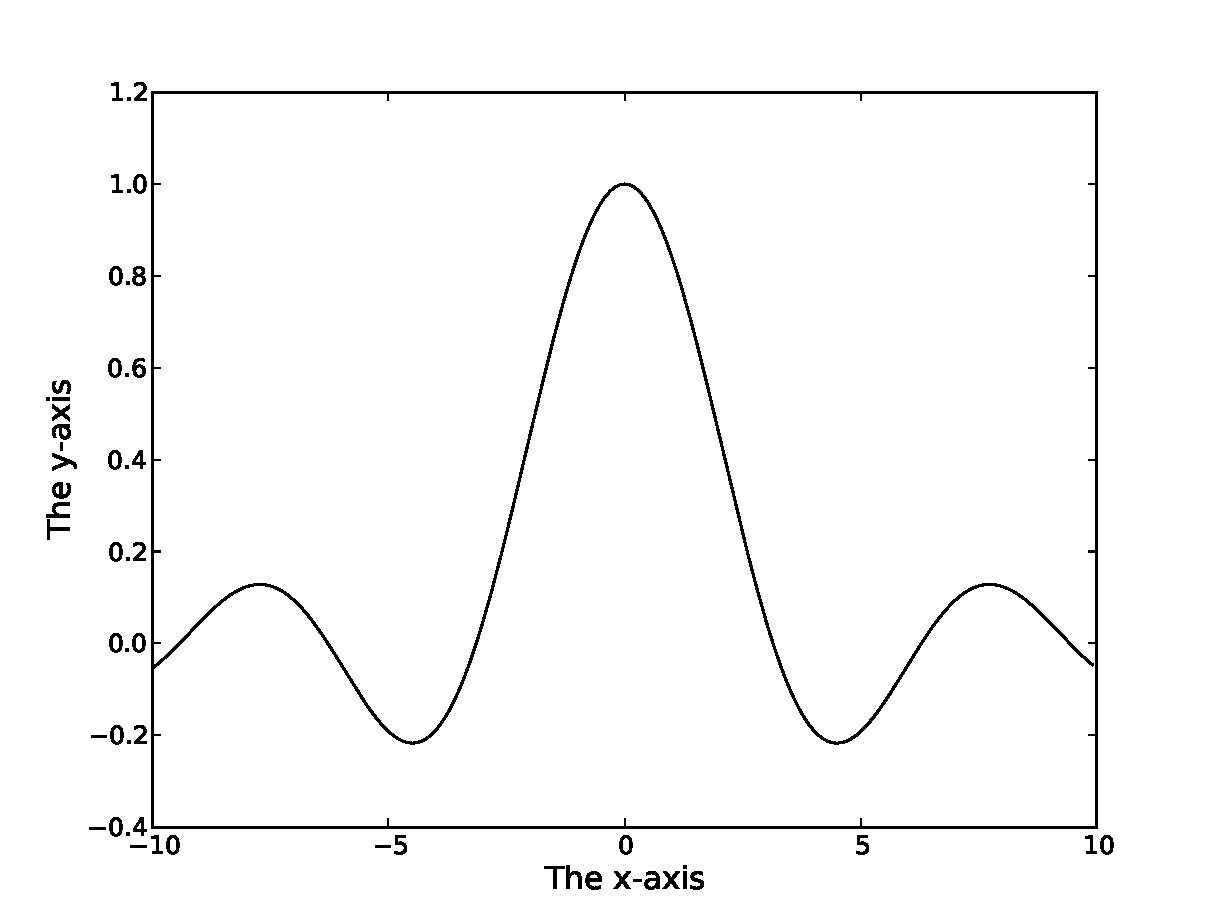
\includegraphics[width=0.5 \textwidth]{figs/sinc1.pdf}
\caption{A $\frac{\sin(x)}{x}$ function.}
\label{fig:vectorFig}
\end{figure}

\section{Units}

When writing units there are a lot of rules and conventions that one has to worry about. These worries can be removed by using the siunitx package, examples of which are given below.

\begin{table}[h!]
\centering
\begin{tabular}{ll}
\toprule
name & unit \\ \midrule
millisecond & \si{ms} \\
meter second & \si{m.s} \\
force & \si{kg.m.s^{-2}}\\
Plank constant & \SI{6.626e-34}{J.s}\\
\bottomrule
\end{tabular}
\end{table}

This is an extremely useful package. Further information on this package can be frond from \url{http://www.texdev.net/wp-content/uploads/2009/12/siunitx.pdf}. 

\section{Tables}

When writing tables use the booktabs package to enhance their readability and neatness. Table \ref{tab:ex} is an example of how to use this package.

\begin{table*}[h!]
\centering
\small
\caption{A test table.}
\begin{tabular}{llrrrrrrrrr}
\toprule
& & \multicolumn{5}{l}{Fitted parameters} & &  & \multicolumn{ 2}{l}{Effected distance} \\ \cmidrule(r){3-7} \cmidrule(r){10-11}
 & & $\beta$ & $A$ & $\alpha$ & $\xi$ & $\omega$ & $R^2$ & RMSE & W-S-W & E-N-E \\ \midrule
\multirow{5}{*}{Ip} & Be & 1.83 & 13.86 & -3.51 & 15.70 & 22.21 & 0.91 & 0.76 & -45.95 & 28.12 \\ 
 & To & 0.36 & 4.08 & -3.13 & 15.01 & 17.73 & 0.93 & 0.16 & -36.44 & 26.83 \\ 
 & Eb & 1.39 & 25.14 & -3.09 & 14.11 & 15.82 & 0.96 & 0.71 & -33.71 & 25.45 \\ 
 & mX & 0.44 & 8.17 & -3.38 & 14.46 & 15.19 & 0.96 & 0.22 & -31.75 & 24.58 \\ 
 & oX & 1.16 & 23.97 & -3.01 & 13.91 & 14.48 & 0.96 & 0.64 & -30.15 & 24.63 \\ \midrule
\multicolumn{2}{l}{Average} & 1.04 & 15.04 & -3.22 & 14.64 & 17.09 & 0.94 & 0.50 & -35.60 & 25.92 \\ 
\multicolumn{2}{l}{Std. Dev} & 0.63 & 9.36 & 0.21 & 0.73 & 3.11 & 0.02 & 0.29 & 6.24 & 1.53 \\ \cmidrule[\heavyrulewidth]{1-11}
\multirow{5}{*}{P} & Be & 0.54 & 4.84 & -5.15 & 22.84 & 34.23 & 0.91 & 0.33 & -64.26 & 34.36 \\ 
 & To & 0.13 & 1.37 & -3.75 & 19.69 & 24.01 & 0.93 & 0.07 & -46.22 & 32.08 \\ 
 & Eb & 0.54 & 8.80 & -2.77 & 16.42 & 18.75 & 0.94 & 0.35 & -37.13 & 30.06 \\ 
 & mX & 0.17 & 2.86 & -2.75 & 16.07 & 17.40 & 0.94 & 0.10 & -34.49 & 29.13 \\ 
 & oX & 0.45 & 8.48 & -2.46 & 15.41 & 16.43 & 0.94 & 0.31 & -32.28 & 29.01 \\ \midrule
\multicolumn{2}{l}{Average}  & 0.37 & 5.27 & -3.38 & 18.09 & 22.16 & 0.93 & 0.23 & -42.88 & 30.93 \\ 
\multicolumn{2}{l}{Std. Dev} & 0.20 & 3.32 & 1.11 & 3.13 & 7.35 & 0.01 & 0.14 & 13.08 & 2.28 \\ \bottomrule
\end{tabular}
\label{tab:ex}
\end{table*}

\section{citations}

For information about the installations requires for the citation packages to work please refer to the \texttt{installationInstructions} file in the \texttt{biblatex-xjenza} folder. When citing there are principally two different ways needed. When the citation is in text, example; \textcite{TestKey} showed that \dots{}. And the normal citation method, example; Research shows that \dots{} \cite{TestKey}.

\printbibliography

\end{document}